\documentclass{beamer}
\usepackage{listings}
\usepackage{xcolor}
\usepackage{tikz}
\usepackage{courier}
\usepackage[utf8]{inputenc}
\usepackage{textcomp}  % For micro symbol

\definecolor{codegreen}{rgb}{0,0.6,0}
\definecolor{codegray}{rgb}{0.5,0.5,0.5}
\definecolor{codepurple}{rgb}{0.58,0,0.82}
\definecolor{backcolour}{rgb}{0.95,0.95,0.95}

\lstdefinestyle{mystyle}{
    backgroundcolor=\color{backcolour},
    commentstyle=\color{codegreen},
    keywordstyle=\color{blue},
    stringstyle=\color{codepurple},
    basicstyle=\ttfamily\footnotesize,
    breakatwhitespace=false,
    breaklines=true,
    captionpos=b,
    keepspaces=true,
    numbersep=5pt,
    showspaces=false,
    showstringspaces=false,
    showtabs=false,
    tabsize=2
}

\lstset{style=mystyle}

\title{Lock-Free Ring Buffer for Market Data}
\author{Low Latency Data Pipeline Team}
\date{\today}

\begin{document}

\begin{frame}
\titlepage
\end{frame}

\begin{frame}{Outline}
\tableofcontents
\end{frame}

\section{Introduction}

\begin{frame}{Why Lock-Free Data Structures?}
\begin{itemize}
    \item \textbf{Challenge}: Modern market data systems process millions of updates per second
    \item \textbf{Problem}: Traditional mutex-based synchronization creates bottlenecks
    \item \textbf{Solution}: Lock-free data structures provide:
    \begin{itemize}
        \item No mutex acquisition/release overhead
        \item No thread blocking
        \item Lower and more predictable latency
        \item Better scalability under contention
    \end{itemize}
    \item \textbf{Application}: Ideal for producer-consumer patterns in market data processing
\end{itemize}
\end{frame}

\section{Ring Buffer Design}

\begin{frame}{Ring Buffer Fundamentals}
\begin{columns}
\column{0.6\textwidth}
    \begin{itemize}
        \item Fixed-size circular buffer
        \item Two atomic indices:
        \begin{itemize}
            \item \texttt{write\_idx\_} - Next position to write
            \item \texttt{read\_idx\_} - Next position to read
        \end{itemize}
        \item Empty when \texttt{read\_idx\_ == write\_idx\_}
        \item Full when \texttt{(write\_idx\_ + 1) \% Size == read\_idx\_}
        \item One slot always reserved for empty detection
    \end{itemize}

\column{0.4\textwidth}
    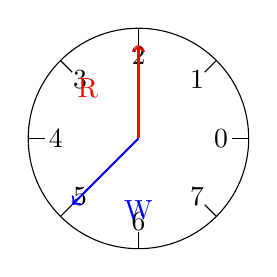
\begin{tikzpicture}[scale=0.7]
        \draw (0,0) circle (2);
        \foreach \i in {0,1,...,7} {
            \draw ({2*cos(45*\i)},{2*sin(45*\i)}) -- ({1.7*cos(45*\i)},{1.7*sin(45*\i)});
            \node at ({1.5*cos(45*\i)},{1.5*sin(45*\i)}) {\i};
        }
        \draw[->, thick, red] (0,0) -- ({1.7*cos(90)},{1.7*sin(90)});
        \node[red] at ({1.3*cos(135)},{1.3*sin(135)}) {R};
        \draw[->, thick, blue] (0,0) -- ({1.7*cos(225)},{1.7*sin(225)});
        \node[blue] at ({1.3*cos(270)},{1.3*sin(270)}) {W};
    \end{tikzpicture}
\end{columns}
\end{frame}

\begin{frame}[fragile]{Implementation Highlights}
\begin{lstlisting}[language=C++]
template <typename T, size_t Size>
class LockFreeRingBuffer {
 public:
  bool TryPush(const T& item) {
    const size_t current_write = write_idx_.load(std::memory_order_relaxed);
    const size_t next_write = (current_write + 1) % Size;
    
    if (next_write == read_idx_.load(std::memory_order_acquire))
      return false;  // Buffer full
    
    buffer_[current_write] = item;
    write_idx_.store(next_write, std::memory_order_release);
    return true;
  }
  
  bool TryPop(T* output) { /* Similar implementation */ }
  
 private:
  alignas(64) std::atomic<size_t> write_idx_{0};
  alignas(64) std::atomic<size_t> read_idx_{0};
  std::array<T, Size> buffer_;
};
\end{lstlisting}
\end{frame}

\begin{frame}{Key Technical Features}
\begin{itemize}
    \item \textbf{Lock-free algorithm}: Using atomic variables
    \item \textbf{Memory ordering}: Careful use of memory ordering constraints
    \begin{itemize}
        \item \texttt{memory\_order\_relaxed} for initial loads
        \item \texttt{memory\_order\_acquire} for checking conditions
        \item \texttt{memory\_order\_release} for committing updates
    \end{itemize}
    \item \textbf{Cache line alignment}: Preventing false sharing between indices
    \begin{itemize}
        \item Producer and consumer threads operate on different cache lines
        \item \texttt{alignas(64)} ensures indices are on separate cache lines
    \end{itemize}
    \item \textbf{Non-blocking behavior}: TryPush/TryPop never block, return boolean success
\end{itemize}
\end{frame}

\section{Testing}

\begin{frame}[fragile]{Basic Functionality Test}
\begin{itemize}
    \item Tests fundamental properties with realistic market data structures:
\begin{lstlisting}[language=C++]
struct MarketTick {
    int64_t timestamp_ns;
    std::string symbol;
    double price;
    double quantity;
    char side;  // 'B' for buy, 'S' for sell
    
    // For testing equality in our assertions
    bool operator==(const MarketTick(*@&@*) other) const;
};
\end{lstlisting}
    \item Verifies:
    \begin{itemize}
        \item Empty buffer detection
        \item Push until full
        \item Pop in FIFO order
        \item Alternating push/pop sequences
    \end{itemize}
\end{itemize}
\end{frame}

\begin{frame}{Market Data Pipeline Test}
\begin{itemize}
    \item Simulates realistic market data processing:
    \begin{itemize}
        \item Producer thread: generates synthetic market tick data
        \item Consumer thread: processes ticks and measures latency
    \end{itemize}
    \item Test parameters:
    \begin{itemize}
        \item 5,000 market ticks
        \item 1024-slot buffer
        \item Alternating BTC/ETH symbols
        \item Realistic price movements
    \end{itemize}
    \item Measures end-to-end latency from tick creation to processing
\end{itemize}
\end{frame}

\begin{frame}{Performance Results}
\begin{columns}
\column{0.5\textwidth}
\begin{itemize}
    \item \textbf{Test machine}: Modern x86\_64 system
    \item \textbf{Compiler}: GCC 13.3.0
    \item \textbf{C++ standard}: C++23
    \item \textbf{Build type}: Release (-O3)
\end{itemize}

\column{0.5\textwidth}
\begin{itemize}
    \item \textbf{Minimum latency}: 215 ns
    \item \textbf{Median latency}: 26,305 ns
    \item \textbf{99th percentile}: 3,284,727 ns
    \item \textbf{Maximum latency}: 4,554,931 ns
\end{itemize}
\end{columns}

\vspace{0.5cm}
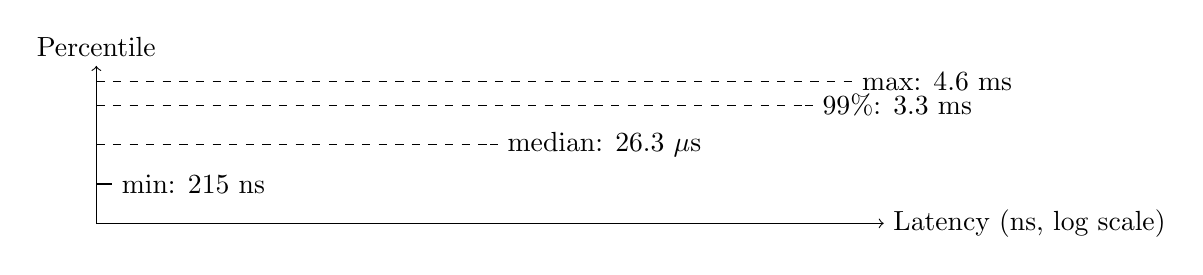
\begin{tikzpicture}
    \draw[->] (0,0) -- (10,0) node[right] {Latency (ns, log scale)};
    \draw[->] (0,0) -- (0,2) node[above] {Percentile};
    
    \draw (0.1,0.5) -- (0.2,0.5) node[right] {min: 215 ns};
    \draw (5,1) -- (5.1,1) node[right] {median: 26.3 $\mu$s};
    \draw (9,1.5) -- (9.1,1.5) node[right] {99\%: 3.3 ms};
    \draw (9.5,1.8) -- (9.6,1.8) node[right] {max: 4.6 ms};
    
    \draw[dashed] (0,0.5) -- (0.1,0.5);
    \draw[dashed] (0,1) -- (5,1);
    \draw[dashed] (0,1.5) -- (9,1.5);
    \draw[dashed] (0,1.8) -- (9.5,1.8);
\end{tikzpicture}
\end{frame}

\section{Applications \& Conclusions}

\begin{frame}{Applications in Market Data Systems}
\begin{itemize}
    \item \textbf{Feed handlers}: Buffering incoming market data packets
    \item \textbf{Parsing pipeline}: Moving raw data to normalization stage
    \item \textbf{Order book updates}: Efficiently queuing price updates
    \item \textbf{Strategy components}: Communicating signals between modules
    \item \textbf{Risk checks}: Queuing pre-trade validations
    \item \textbf{Logging}: Non-blocking capture of events for later analysis
\end{itemize}
\end{frame}

\begin{frame}{Conclusions \& Next Steps}
\begin{itemize}
    \item \textbf{Achievements}:
    \begin{itemize}
        \item Created a fully lock-free, high-performance ring buffer
        \item Demonstrated functionality with real market data structures
        \item Measured sub-microsecond minimum latency
        \item Successfully processed thousands of events with predictable performance
    \end{itemize}
    \item \textbf{Potential improvements}:
    \begin{itemize}
        \item Multi-producer/multi-consumer variants
        \item Batched operations for higher throughput
        \item Memory reclamation for dynamically allocated elements
        \item Integration with hardware acceleration (FPGA, GPU)
    \end{itemize}
\end{itemize}
\end{frame}

\begin{frame}{Thank You}
\centering
\Huge{Questions?}

\vspace{1cm}
\normalsize
Our implementation is available in the project repository:\\
\texttt{src/core/ring\_buffer.h}
\end{frame}

\end{document}